\documentclass[12pt,a4paper]{article}

% ─── Page Layout ───────────────────────────────────────────────────────────────
\usepackage[a4paper, margin=0.8in, headheight=14pt]{geometry}

% ─── Fonts (XeLaTeX) ───────────────────────────────────────────────────────────
\usepackage{fontspec}
\usepackage{unicode-math}
\setmainfont{TeX Gyre Pagella}
\setmonofont[Scale=0.88]{TeX Gyre Cursor}
\setmathfont{Latin Modern Math}

% ─── Packages ──────────────────────────────────────────────────────────────────
\usepackage{xcolor}
\usepackage{colortbl}
\usepackage{titlesec}
\usepackage{enumitem}
\usepackage{tabularx}
\usepackage{booktabs}
\usepackage{array}
\usepackage{amsmath}
\usepackage{tikz}
\usetikzlibrary{shapes.geometric, arrows.meta, positioning, calc, fit, decorations.pathreplacing, patterns}
\usepackage{tcolorbox}
\tcbuselibrary{skins, breakable}
\usepackage{hyperref}
\usepackage{fancyhdr}
\usepackage{graphicx}
\usepackage{microtype}
\hyphenpenalty=10000
\exhyphenpenalty=10000
\sloppy
\usepackage{caption}
\usepackage{setspace}
\usepackage{multirow}
\usepackage{tocloft}

% ─── Q&A helper ────────────────────────────────────────────────────────────────
\newcommand{\Q}[1]{\textbf{#1}\par\noindent\ignorespaces}

% ─── Colour Palette ────────────────────────────────────────────────────────────
\definecolor{myred}{RGB}{196,30,58}
\definecolor{mydark}{RGB}{30,30,50}
\definecolor{mygreen}{RGB}{14,120,80}
\definecolor{myteal}{RGB}{0,130,140}
\definecolor{myamber}{RGB}{180,100,0}
\definecolor{mypurple}{RGB}{100,30,160}
\definecolor{mygray}{RGB}{246,247,249}
\definecolor{mgframe}{RGB}{180,185,200}
\definecolor{watermark}{RGB}{145,150,170}
\definecolor{hdrred}{RGB}{250,232,235}
\definecolor{hdrgreen}{RGB}{220,244,233}
\definecolor{hdrteal}{RGB}{220,242,244}
\definecolor{hdramber}{RGB}{253,242,215}
\definecolor{hdrpurple}{RGB}{238,228,255}
\definecolor{hdrgray}{RGB}{238,240,245}
\definecolor{rowalt}{RGB}{250,251,253}

% ─── Section Formatting ────────────────────────────────────────────────────────
\titleformat{\section}
  {\large\bfseries\color{myred}}{\thesection.}{0.5em}{}
  [\vspace{1pt}{\color{myred}\rule{\linewidth}{0.8pt}}]
\titleformat{\subsection}
  {\normalsize\bfseries\color{myteal}}{\thesubsection}{0.5em}{}
\titlespacing*{\section}{0pt}{18pt}{7pt}
\titlespacing*{\subsection}{0pt}{11pt}{4pt}

% ─── Paragraph ─────────────────────────────────────────────────────────────────
\setlength{\parindent}{0pt}
\setlength{\parskip}{4pt}

% ─── TOC Styling ───────────────────────────────────────────────────────────────
\renewcommand{\cfttoctitlefont}{\large\bfseries\color{myred}}
\renewcommand{\cftaftertoctitle}{\par\noindent{\color{myred}\rule{\linewidth}{0.8pt}}}
\setlength{\cftbeforetoctitleskip}{0pt}
\setlength{\cftaftertoctitleskip}{6pt}
\renewcommand{\cftsecfont}{\normalsize\bfseries\color{mydark}}
\renewcommand{\cftsecpagefont}{\normalsize\bfseries\color{mydark}}
\renewcommand{\cftsecleader}{\cftdotfill{\cftdotsep}}
\setlength{\cftbeforesecskip}{7pt}
\renewcommand{\cftsubsecfont}{\small\color{mydark}}
\renewcommand{\cftsubsecpagefont}{\small\color{mydark}}
\setlength{\cftbeforesubsecskip}{3pt}
\setlength{\cftsubsecindent}{1.4em}

% ─── Table helpers ─────────────────────────────────────────────────────────────
\renewcommand{\arraystretch}{1.45}
\setlength{\tabcolsep}{6pt}
\arrayrulecolor{mydark}
\newcolumntype{B}[1]{>{\small\bfseries\raggedright\arraybackslash}m{#1}}
\newcolumntype{Y}{>{\small\raggedright\arraybackslash}X}
\renewcommand{\tabularxcolumn}[1]{m{#1}}

% ─── Header / Footer ───────────────────────────────────────────────────────────
\pagestyle{fancy}
\fancyhf{}
\fancyhead[L]{\small\color{myred}\textbf{ES-CS301}\;\color{mydark}--- Data Structure \& Algorithms}
\fancyhead[R]{\small\color{myteal}\textbf{Module 3 Notes}}
\fancyfoot[C]{\small\color{mydark}\thepage}
\fancyfoot[R]{\small\color{watermark}\textit{\copyright\ Biraj}}
\renewcommand{\headrulewidth}{0.5pt}
\renewcommand{\footrulewidth}{0.3pt}

% ─── Hyperref ──────────────────────────────────────────────────────────────────
\hypersetup{
  colorlinks=true, linkcolor=myteal, urlcolor=myteal,
  pdfauthor={Biraj Sarkar (CGEC)},
  pdftitle={ES-CS301 --- Module 3 Notes: Linked Lists and Tree Data Structures}
}

% ─── tcolorbox styles ──────────────────────────────────────────────────────────
\tcbset{
  tikzbox/.style={
    colback=mygray, colframe=mgframe, boxrule=0.6pt, arc=4pt,
    left=8pt, right=8pt, top=6pt, bottom=6pt,
    colbacktitle=mgframe, coltitle=mydark,
    fonttitle=\small\bfseries
  },
  defbox/.style={
    colback=hdrgreen, colframe=mygreen, boxrule=0.8pt, arc=4pt,
    left=9pt, right=9pt, top=6pt, bottom=6pt,
    colbacktitle=mygreen, coltitle=white,
    fonttitle=\small\bfseries
  },
  formulabox/.style={
    colback=hdrteal, colframe=myteal, boxrule=0.8pt, arc=4pt,
    left=9pt, right=9pt, top=7pt, bottom=7pt,
    colbacktitle=myteal, coltitle=white,
    fonttitle=\small\bfseries
  },
  examplebox/.style={
    colback=hdramber, colframe=myamber, boxrule=0.8pt, arc=4pt,
    left=9pt, right=9pt, top=6pt, bottom=6pt,
    colbacktitle=myamber, coltitle=white,
    fonttitle=\small\bfseries
  },
  masonbox/.style={
    colback=hdrpurple, colframe=mypurple, boxrule=0.8pt, arc=4pt,
    left=9pt, right=9pt, top=6pt, bottom=6pt,
    colbacktitle=mypurple, coltitle=white,
    fonttitle=\small\bfseries
  },
  exambox/.style={
    colback=hdrpurple, colframe=mypurple, boxrule=1pt, arc=5pt,
    left=10pt, right=10pt, top=8pt, bottom=8pt,
    colbacktitle=mypurple, coltitle=white,
    fonttitle=\bfseries,
    breakable, title after break={\textbf{Frequently Asked / Viva Questions (contd.)}}
  }
}

\tcbset{breakable}
\tcbset{after={\color{black}}}

% ─── TikZ styles ───────────────────────────────────────────────────────────────
\tikzset{
  llnode/.style={rectangle, draw=myteal, fill=hdrteal, minimum width=1.6cm, minimum height=0.7cm, font=\small, align=center},
  treenode/.style={circle, draw=myred, fill=hdrred, font=\small\bfseries, inner sep=2pt, minimum size=0.8cm},
  arrow/.style={-Stealth, thick, color=mydark},
  redarrow/.style={-Stealth, thick, color=myred},
  line/.style={thick, color=mydark}
}

\begin{document}

% ─── Title Page ───────────────────────────────────────────────────────────────
\begin{center}
  {\LARGE\bfseries\color{myred} ES-CS301 --- Data Structure \& Algorithms}\\[5pt]
  {\normalsize\color{mydark} Semester III \quad$\bullet$\quad 3L:0T:4P \quad$\bullet$\quad 3 Credits}\\[3pt]
  {\normalsize\color{myteal}\textbf{Module 3 Exam Notes: Linked Lists and Tree Data Structures}}\\[3pt]
  {\small\color{mydark} CGEC \;$|$\; B.Tech ECE (2023--27) \;$|$\; \textit{Biraj Sarkar}}
\end{center}
\vspace{2pt}
\noindent{\color{myred}\rule{\linewidth}{1.5pt}}
\vspace{2pt}

\hypersetup{linkcolor=mydark}
\tableofcontents
\hypersetup{linkcolor=myteal}
\newpage

% ───────────────────────────────────────────────────────────────────────────────
\section{Linked Lists Fundamentals and Singly Linked List (SLL)}
% ───────────────────────────────────────────────────────────────────────────────

\begin{tcolorbox}[defbox, title={\textbf{Definition: Singly Linked List (SLL) Architecture}}]
A \textbf{Singly Linked List} is a dynamic linear data structure composed of distinct nodes allocated at arbitrary non-contiguous physical memory locations. Each node consists of two essential components:
\begin{enumerate}[leftmargin=*, nosep]
  \item \textbf{Data Field:} Stores the actual information payload of type $T$.
  \item \textbf{Link (Next Pointer):} Stores the explicit physical memory address of the logically succeeding node.
\end{enumerate}
The list is anchored by an external pointer \texttt{head} referencing the first node. The terminal node's link contains \texttt{NULL}.
\end{tcolorbox}

\subsection{Limitations of Arrays vs Advantages of Linked Lists}
\begin{itemize}[leftmargin=*, itemsep=3pt]
  \item \textbf{Memory Allocation:} Arrays require fixed, compile-time contiguous memory allocation. Linked lists allocate memory dynamically on the heap at runtime via \texttt{malloc()} / \texttt{free()}, growing and shrinking on demand.
  \item \textbf{Insertion and Deletion Overhead:} Inserting or deleting an element at index $0$ in an array of size $n$ requires shifting all $n$ subsequent elements ($\mathcal{O}(n)$ time). In a linked list, inserting or deleting at the head requires updating pointer references, which executes in strictly $\mathbf{\mathcal{O}(1)}$ time without moving physical payloads.
  \item \textbf{Memory Fragmentation:} Arrays can suffer allocation failure due to external memory fragmentation even when total free RAM exceeds the array size; linked lists utilize scattered memory chunks effectively.
\end{itemize}

\begin{tcolorbox}[tikzbox, title={\textbf{Memory Representation and Pointer Rewiring in a Singly Linked List}}]
\centering
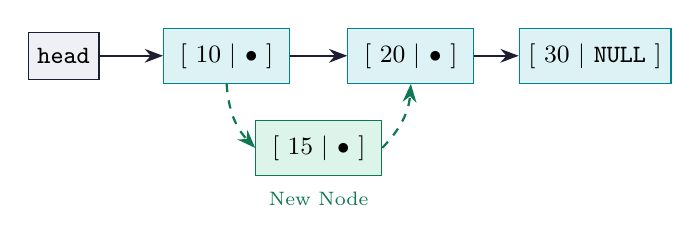
\begin{tikzpicture}[every node/.style={font=\small}, scale=0.9]
  % Head pointer
  \node[draw=mydark, fill=hdrgray, minimum size=0.6cm] (head) at (-1.5,0) {\texttt{head}};
  \node[llnode] (n1) at (0.8,0) {[ 10 $|$ $\bullet$ ]};
  \node[llnode] (n2) at (3.4,0) {[ 20 $|$ $\bullet$ ]};
  \node[llnode] (n3) at (6.0,0) {[ 30 $|$ \texttt{NULL} ]};

  \draw[arrow] (head) -- (n1.west);
  \draw[arrow] (n1.east) -- (n2.west);
  \draw[arrow] (n2.east) -- (n3.west);

  % Insertion example
  \node[llnode, draw=mygreen, fill=hdrgreen] (new) at (2.1,-1.3) {[ 15 $|$ $\bullet$ ]};
  \node[below=2pt, font=\scriptsize, color=mygreen] at (2.1,-1.7) {New Node};
  \draw[-Stealth, thick, color=mygreen, dashed] (n1.south) to[bend right=20] (new.west);
  \draw[-Stealth, thick, color=mygreen, dashed] (new.east) to[bend right=20] (n2.south);
\end{tikzpicture}
\end{tcolorbox}

\subsection{Singly Linked List Algorithmic Operations}
\begin{tcolorbox}[formulabox, title={\textbf{Algorithms for Insertion and Deletion in SLL}}]
\textbf{1. Insertion at Beginning ($\mathcal{O}(1)$):}
\begin{verbatim}
newNode = allocateNode(val);
newNode->next = head;
head = newNode;
\end{verbatim}

\textbf{2. Insertion at End ($\mathcal{O}(n)$ without tail pointer, $\mathcal{O}(1)$ with tail):}
\begin{verbatim}
newNode = allocateNode(val); newNode->next = NULL;
if (head == NULL) { head = newNode; return; }
ptr = head;
while (ptr->next != NULL) ptr = ptr->next;
ptr->next = newNode;
\end{verbatim}

\textbf{3. Deletion at Beginning ($\mathcal{O}(1)$):}
\begin{verbatim}
if (head == NULL) report "Underflow";
temp = head;
head = head->next;
free(temp);
\end{verbatim}

\textbf{4. Deletion of a Node with Value $X$ ($\mathcal{O}(n)$):}
\begin{verbatim}
if (head == NULL) return;
if (head->data == X) { temp = head; head = head->next; free(temp); return; }
curr = head; prev = NULL;
while (curr != NULL && curr->data != X) { prev = curr; curr = curr->next; }
if (curr == NULL) report "Key Not Found";
else { prev->next = curr->next; free(curr); }
\end{verbatim}
\end{tcolorbox}

% ───────────────────────────────────────────────────────────────────────────────
\section{Linked Representation of Stack and Queue \& Header Nodes}
% ───────────────────────────────────────────────────────────────────────────────

\subsection{Linked Stack and Linked Queue}
\begin{itemize}[leftmargin=*, itemsep=3pt]
  \item \textbf{Linked Stack:} Implemented by inserting and deleting strictly at the head node of the linked list:
  \begin{itemize}[leftmargin=*, nosep]
    \item $\text{Push}(x) \equiv \text{Insert at Beginning} \implies \mathbf{\mathcal{O}(1)}$
    \item $\text{Pop}() \equiv \text{Delete from Beginning} \implies \mathbf{\mathcal{O}(1)}$
    \item Overflow never occurs unless the system runs out of heap memory.
  \end{itemize}
  \item \textbf{Linked Queue:} Maintained via two external pointers: \texttt{front} and \texttt{rear}:
  \begin{itemize}[leftmargin=*, nosep]
    \item $\text{Enqueue}(x) \equiv \text{Insert at End (via \texttt{rear}->\texttt{next} = newNode; \texttt{rear} = newNode)} \implies \mathbf{\mathcal{O}(1)}$
    \item $\text{Dequeue}() \equiv \text{Delete at Head (via \texttt{front} = \texttt{front}->\texttt{next})} \implies \mathbf{\mathcal{O}(1)}$
  \end{itemize}
\end{itemize}

\subsection{Header Nodes in Linked Lists}
A \textbf{Header Node} is a dummy node placed at the very beginning of the linked list before the first actual data node:
\begin{itemize}[leftmargin=*, itemsep=2pt]
  \item \textbf{Grounded Header List:} Header node's link points to the first data node; the last node's link contains \texttt{NULL}.
  \item \textbf{Circular Header List:} The last node's link points back to the header node itself.
  \item \textbf{Key Advantages:}
  \begin{enumerate}[leftmargin=*, nosep]
    \item Eliminates special-case coding for operations at the head (head pointer never needs re-assignment).
    \item The list is never truly empty (\texttt{head != NULL} always holds; an empty list has \texttt{head->next == NULL} or \texttt{head->next == head}).
    \item The header node's data field can store metadata (e.g., total node count, maximum element).
  \end{enumerate}
\end{itemize}

% ───────────────────────────────────────────────────────────────────────────────
\section{Doubly Linked Lists (DLL) and Circular Linked Lists (CLL)}
% ───────────────────────────────────────────────────────────────────────────────

\subsection{Doubly Linked List (DLL)}
In a \textbf{Doubly Linked List}, each node contains three fields: \texttt{prev} pointer, \texttt{data}, and \texttt{next} pointer.
\par\vspace{4pt}
\begin{itemize}[leftmargin=*, itemsep=3pt]
  \item \textbf{Invariant:} $\texttt{p->next->prev} == \texttt{p}$ and $\texttt{p->prev->next} == \texttt{p}$.
  \item \textbf{Bidirectional Traversal:} Allows forward and reverse scanning from any arbitrary node.
  \item \textbf{$\mathcal{O}(1)$ Deletion Given Node Pointer:} Deleting node $P$ does not require searching for its predecessor:
  \begin{verbatim}
  P->prev->next = P->next;
  if (P->next != NULL) P->next->prev = P->prev;
  free(P);
  \end{verbatim}
  \item \textbf{Trade-off:} Extra memory overhead for backward pointers ($2\times$ pointer overhead per node) and additional pointer adjustments during insertions.
\end{itemize}

\subsection{Circular Linked Lists (CLL)}
In a \textbf{Circular Singly Linked List}, the last node's link points back to the first node.
\par\vspace{3pt}
\begin{itemize}[leftmargin=*, itemsep=3pt]
  \item \textbf{Tail Pointer Paradigm:} By maintaining a single pointer \texttt{tail} to the last node:
  \begin{itemize}[leftmargin=*, nosep]
    \item Last node is accessible in $\mathcal{O}(1)$ (\texttt{tail}).
    \item First node is accessible in $\mathcal{O}(1)$ (\texttt{tail->next}).
    \item Both insertion at head and insertion at tail execute in strictly $\mathbf{\mathcal{O}(1)}$ time!
  \end{itemize}
  \item \textbf{Applications:} Continuous cycling processes, round-robin CPU scheduling, multiplayer turn games.
\end{itemize}

\subsection{Polynomial Representation and Addition using Linked Lists}
A single-variable polynomial $P(x) = a_n x^{e_n} + a_{n-1} x^{e_{n-1}} + \dots + a_0 x^{e_0}$ is represented as a linked list where each node contains: \texttt{coeff} (coefficient), \texttt{exp} (exponent), and \texttt{next} pointer, maintained in strictly decreasing order of exponents.

\begin{tcolorbox}[defbox, title={\textbf{Algorithm: Polynomial Addition using Singly Linked Lists}}]
\textbf{Algorithm AddPolynomials($P_1, P_2$):}
\begin{enumerate}[leftmargin=*, nosep]
  \item Initialize pointers $p = P_1, \; q = P_2$, and an empty resultant list $P_3$.
  \item While $p \ne \text{NULL}$ and $q \ne \text{NULL}$:
  \begin{itemize}[leftmargin=*, nosep]
    \item \textbf{Case 1 ($p\to\text{exp} == q\to\text{exp}$):} Compute $\text{sum} = p\to\text{coeff} + q\to\text{coeff}$. If $\text{sum} \ne 0$, insert term $(\text{sum}, p\to\text{exp})$ into $P_3$. Advance $p = p\to\text{next}, \; q = q\to\text{next}$.
    \item \textbf{Case 2 ($p\to\text{exp} > q\to\text{exp}$):} Insert term $(p\to\text{coeff}, p\to\text{exp})$ into $P_3$. Advance $p = p\to\text{next}$.
    \item \textbf{Case 3 ($p\to\text{exp} < q\to\text{exp}$):} Insert term $(q\to\text{coeff}, q\to\text{exp})$ into $P_3$. Advance $q = q\to\text{next}$.
  \end{itemize}
  \item Copy any remaining terms from $p$ or $q$ to the tail of $P_3$. Return $P_3$.
\end{enumerate}
Time Complexity: $\mathbf{\mathcal{O}(m + n)}$ where $m, n$ are the number of non-zero terms in $P_1, P_2$.
\end{tcolorbox}

% ───────────────────────────────────────────────────────────────────────────────
\section{Tree Terminologies and Binary Tree Foundations}
% ───────────────────────────────────────────────────────────────────────────────

\begin{tcolorbox}[defbox, title={\textbf{Definition: Tree Data Structure and Core Terminologies}}]
A \textbf{Tree} is a non-linear, hierarchical data structure consisting of a collection of nodes connected by directed or undirected edges, such that there exists a unique root node $R$ and no cycles.
\par\vspace{4pt}
\begin{itemize}[leftmargin=*, itemsep=2pt]
  \item \textbf{Root:} The topmost ancestor node with in-degree 0 (no incoming parent edge).
  \item \textbf{Leaf (Terminal Node):} A node with out-degree 0 (no child nodes).
  \item \textbf{Degree of a Node:} The total number of subtrees or immediate children attached to that node.
  \item \textbf{Degree of a Tree:} The maximum degree among all nodes in the tree.
  \item \textbf{Level and Depth:} The root is at Level 0 (or 1). The depth of a node is the length of the path from the root to that node.
  \item \textbf{Height of a Tree ($h$):} The maximum depth among all nodes in the tree (length of the longest path from root to leaf).
\end{itemize}
\end{tcolorbox}

\subsection{Mathematical Properties of Binary Trees}
A \textbf{Binary Tree} is a finite tree in which every node has at most two children, distinguished as \textbf{left child} and \textbf{right child}.
\begin{tcolorbox}[formulabox, title={\textbf{Core Mathematical Theorems on Binary Trees}}]
\begin{enumerate}[leftmargin=*, itemsep=3pt]
  \item Maximum number of nodes at level $i$ (with root at level 0):
  \begin{equation}
    N_{\max}(i) = 2^i
  \end{equation}
  \item Maximum total nodes in a binary tree of height $h$:
  \begin{equation}
    N_{\max}(h) = \sum_{i=0}^h 2^i = 2^{h+1} - 1
  \end{equation}
  \item Minimum height of a binary tree with $n$ nodes:
  \begin{equation}
    h_{\min} = \lceil \log_2(n + 1) \rceil - 1
  \end{equation}
  \item \textbf{Leaf vs Degree-2 Nodes Theorem:} In any non-empty binary tree, the number of leaf nodes $n_0$ is exactly one more than the number of nodes with degree two ($n_2$):
  \begin{equation}
    \mathbf{n_0 = n_2 + 1}
  \end{equation}
  \textit{Proof:} Let total nodes be $n = n_0 + n_1 + n_2$. Total edges in a tree of $n$ nodes is $E = n - 1$. Also, each degree-1 node contributes 1 outgoing branch and each degree-2 node contributes 2 outgoing branches: $E = n_1 + 2n_2$. Equating the two expressions:
  \begin{equation*}
    n_0 + n_1 + n_2 - 1 = n_1 + 2n_2 \implies n_0 - 1 = n_2 \implies \mathbf{n_0 = n_2 + 1}
  \end{equation*}
\end{enumerate}
\end{tcolorbox}

\subsection{Binary Tree Classifications}
\begin{itemize}[leftmargin=*, itemsep=3pt]
  \item \textbf{Full (Strict / Proper) Binary Tree:} Every internal node has exactly two children ($0$ or $2$ children; no node has degree 1).
  \item \textbf{Complete Binary Tree:} All levels are completely filled except possibly the last level, where nodes are filled strictly from left to right without gaps. Foundation of array-based Binary Heaps.
  \item \textbf{Perfect Binary Tree:} All internal nodes have two children and all leaves reside at the same maximum depth (contains exactly $2^{h+1}-1$ nodes).
  \item \textbf{Degenerate (Skewed) Binary Tree:} Every internal node has only one child, degrading to a linear linked list ($\mathcal{O}(n)$ height).
\end{itemize}

\subsection{Binary Tree Traversals}
\begin{enumerate}[leftmargin=*, itemsep=3pt]
  \item \textbf{Preorder Traversal (D-L-R):} Process Data $\to$ Traverse Left subtree $\to$ Traverse Right subtree.
  \item \textbf{Inorder Traversal (L-D-R):} Traverse Left subtree $\to$ Process Data $\to$ Traverse Right subtree. Produces sorted sequence for a BST!
  \item \textbf{Postorder Traversal (L-R-D):} Traverse Left subtree $\to$ Traverse Right subtree $\to$ Process Data. Used for deleting tree bottom-up and expression evaluation.
  \item \textbf{Level-Order Traversal (BFS):} Visit nodes level by level from top to bottom, left to right, implemented using a FIFO Queue.
\end{enumerate}

% ───────────────────────────────────────────────────────────────────────────────
\section{Threaded Binary Tree}
% ───────────────────────────────────────────────────────────────────────────────

\begin{tcolorbox}[defbox, title={\textbf{Definition: Threaded Binary Tree}}]
In an $n$-node binary tree, exactly $2n$ pointer fields exist, of which $n-1$ point to children and $n+1$ are \texttt{NULL}. A \textbf{Threaded Binary Tree} utilizes these wasted null pointers:
\begin{itemize}[leftmargin=*, nosep]
  \item A \texttt{NULL} left pointer is converted into a \textbf{thread} pointing to the node's \textbf{Inorder Predecessor}.
  \item A \texttt{NULL} right pointer is converted into a \textbf{thread} pointing to the node's \textbf{Inorder Successor}.
\end{itemize}
Boolean tags (\texttt{lTag}, \texttt{rTag}) indicate whether the pointer field is a normal child link ($0$) or a thread ($1$).
\end{tcolorbox}

\textbf{Primary Advantage:} Enables complete Inorder traversal without requiring recursive calls or an auxiliary stack, utilizing $\mathbf{\mathcal{O}(1)}$ auxiliary memory space.

% ───────────────────────────────────────────────────────────────────────────────
\section{Binary Search Tree (BST)}
% ───────────────────────────────────────────────────────────────────────────────

\begin{tcolorbox}[defbox, title={\textbf{Definition: Binary Search Tree (BST) Invariant}}]
A \textbf{Binary Search Tree (BST)} is a binary tree in which every node $x$ satisfies the BST ordering property:
\begin{itemize}[leftmargin=*, nosep]
  \item For all nodes $y$ in the left subtree of $x$: $\text{Key}(y) < \text{Key}(x)$.
  \item For all nodes $z$ in the right subtree of $x$: $\text{Key}(z) > \text{Key}(x)$.
\end{itemize}
Duplicate keys are either disallowed or handled uniformly in right subtrees.
\end{tcolorbox}

\subsection{BST Operations and Recursive Algorithms}
\begin{tcolorbox}[formulabox, title={\textbf{Core Binary Search Tree Algorithms}}]
\textbf{1. Algorithm BST\_Search($root, K$):}
\begin{verbatim}
if (root == NULL || root->data == K) return root;
if (K < root->data) return BST_Search(root->left, K);
return BST_Search(root->right, K);
\end{verbatim}

\textbf{2. Algorithm BST\_Insert($root, K$):}
\begin{verbatim}
if (root == NULL) return createNode(K);
if (K < root->data) root->left = BST_Insert(root->left, K);
else if (K > root->data) root->right = BST_Insert(root->right, K);
return root;
\end{verbatim}

\textbf{3. Algorithm BST\_Delete($root, K$):}
\begin{verbatim}
if (root == NULL) return root;
if (K < root->data) root->left = BST_Delete(root->left, K);
else if (K > root->data) root->right = BST_Delete(root->right, K);
else {
    // Case 1: Leaf node or Case 2: One child
    if (root->left == NULL) {
        temp = root->right; free(root); return temp;
    } else if (root->right == NULL) {
        temp = root->left; free(root); return temp;
    }
    // Case 3: Two children
    temp = findMin(root->right); // Inorder Successor
    root->data = temp->data;
    root->right = BST_Delete(root->right, temp->data);
}
return root;
\end{verbatim}
Complexity: Average $\mathbf{\mathcal{O}(\log_2 n)}$, Worst (skewed tree) $\mathbf{\mathcal{O}(n)}$.
\end{tcolorbox}

% ───────────────────────────────────────────────────────────────────────────────
\section{AVL Tree (Self-Balancing Binary Search Tree)}
% ───────────────────────────────────────────────────────────────────────────────

\begin{tcolorbox}[defbox, title={\textbf{Definition: AVL Tree and Balance Factor}}]
An \textbf{AVL Tree} is a strictly height-balanced Binary Search Tree where the \textbf{Balance Factor ($BF$)} of every node $v$ is constrained to $\{-1, 0, +1\}$:
\begin{equation}
  BF(v) = h(\text{left subtree}) - h(\text{right subtree}) \in \{-1, 0, +1\}
\end{equation}
If an insertion or deletion causes $|BF(v)| \ge 2$, the tree is rebalanced locally via rotations.
\end{tcolorbox}

\subsection{AVL Rebalancing Rotations}
\begin{enumerate}[leftmargin=*, itemsep=4pt]
  \item \textbf{LL Rotation (Single Right Rotation):} Applied when insertion occurs in the left subtree of the left child ($BF = +2$, child $BF = +1$).
  \item \textbf{RR Rotation (Single Left Rotation):} Applied when insertion occurs in the right subtree of the right child ($BF = -2$, child $BF = -1$).
  \item \textbf{LR Rotation (Double Rotation):} Insertion in the right subtree of the left child ($BF = +2$, child $BF = -1$). First Left-rotate left child, then Right-rotate parent.
  \item \textbf{RL Rotation (Double Rotation):} Insertion in the left subtree of the right child ($BF = -2$, child $BF = +1$). First Right-rotate right child, then Left-rotate parent.
\end{enumerate}

\begin{tcolorbox}[examplebox, title={\textbf{Step-by-Step AVL Construction Walkthrough}}]
Construct an AVL tree by inserting keys: $10, 20, 30, 40, 50, 25$.
\begin{itemize}[leftmargin=*, nosep]
  \item Insert $10, 20$: Tree balanced.
  \item Insert $30$: Path $10 \to 20 \to 30$ causes $BF(10) = -2$ (RR violation). Perform \textbf{RR (Left Rotation)} on $10$: $20$ becomes root, with children $10$ (left) and $30$ (right).
  \item Insert $40$: Attached as right child of $30$. Balanced ($BF(20)=-1$).
  \item Insert $50$: Path $30 \to 40 \to 50$ causes $BF(30) = -2$ (RR violation). Perform \textbf{RR (Left Rotation)} on $30$: $40$ takes $30$'s position, children $30, 50$.
  \item Insert $25$: Attached as left child of $30$. Root $20$ now has $BF(20) = -2$, child $40$ has $BF(40) = +1$ (RL violation). Perform \textbf{RL Double Rotation}: Right-rotate $40$ then Left-rotate $20$. New root is $30$, left subtree rooted at $20$ (children $10, 25$), right subtree rooted at $40$ (child $50$). Tree is perfectly balanced!
\end{itemize}
\end{tcolorbox}

\begin{tcolorbox}[formulabox, title={\textbf{Height Bound and Complexity of AVL Trees}}]
The minimum number of nodes $N(h)$ in an AVL tree of height $h$ satisfies the Fibonacci recurrence:
\begin{equation}
  N(h) = N(h-1) + N(h-2) + 1, \quad N(0) = 1, \; N(1) = 2
\end{equation}
Solving this relation yields an asymptotic upper bound on height:
\begin{equation}
  h < 1.44 \log_2(n + 2) \implies \mathbf{h = \mathcal{O}(\log_2 n)}
\end{equation}
Consequently, Search, Insert, and Delete operations in an AVL tree are \textbf{guaranteed strictly $\mathbf{\mathcal{O}(\log n)}$} in both average and worst cases!
\end{tcolorbox}

% ───────────────────────────────────────────────────────────────────────────────
\section{Applications of Binary Trees: Expression Trees and Huffman Coding}
% ───────────────────────────────────────────────────────────────────────────────

\subsection{Expression Trees}
An \textbf{Expression Tree} is a binary tree representing an arithmetic or logical formula:
\begin{itemize}[leftmargin=*, nosep]
  \item \textbf{Leaves:} Distinct operands (variables or numerical constants).
  \item \textbf{Internal Nodes:} Binary operators ($+, -, *, /, \wedge$).
  \item \textbf{Traversals:} Inorder traversal with parentheses yields the equivalent \textbf{Infix} formula; Preorder traversal yields \textbf{Prefix}; Postorder traversal yields \textbf{Postfix}.
  \item \textbf{Construction Algorithm from Postfix:} Scan postfix expression token by token using a stack of tree node pointers. For an operand, create a leaf node and push pointer. For operator $\odot$, create an operator node, pop two nodes as right and left children, and push the newly formed subtree.
\end{itemize}

\subsection{Huffman Coding (Greedy Data Compression)}
\begin{tcolorbox}[defbox, title={\textbf{Huffman Algorithm for Optimal Prefix Codes}}]
Given an alphabet of $n$ symbols with given occurrence frequencies:
\begin{enumerate}[leftmargin=*, nosep]
  \item Create a Min-Priority Queue containing $n$ leaf nodes, each initialized with a symbol and its frequency.
  \item While the priority queue contains more than one node:
  \begin{itemize}[leftmargin=*, nosep]
    \item $left = \text{Extract-Min}()$
    \item $right = \text{Extract-Min}()$
    \item Allocate a new internal node $Z$ with $\text{freq}(Z) = \text{freq}(left) + \text{freq}(right)$.
    \item Set $Z\to\text{left} = left$ and $Z\to\text{right} = right$.
    \item $\text{Insert}(Z)$ back into the Min-Priority Queue.
  \end{itemize}
  \item The remaining single node is the root of the \textbf{Huffman Tree}.
  \item Assign binary bit \texttt{'0'} to each left branch and \texttt{'1'} to each right branch. Paths from root to leaves produce unambiguous \textbf{Prefix Codes} (no code is a prefix of another).
\end{enumerate}
Time Complexity: $\mathbf{\mathcal{O}(n \log_2 n)}$ using a binary min-heap.
\end{tcolorbox}

% ───────────────────────────────────────────────────────────────────────────────
\section{Multi-Way Search Trees: B-Tree and B+ Tree}
% ───────────────────────────────────────────────────────────────────────────────

\subsection{B-Tree of Order $m$}
Designed for secondary storage (disk systems) to minimize slow disk I/O operations by maximizing node branching factor.
\begin{tcolorbox}[defbox, title={\textbf{Axiomatic Properties of B-Tree of Order $m$}}]
\begin{enumerate}[leftmargin=*, nosep]
  \item Every node has at most $m$ children and $m - 1$ keys.
  \item The root node has at least $2$ children (unless it is a leaf).
  \item Every internal node (except root) has at least $\lceil m/2 \rceil$ children and $\lceil m/2 \rceil - 1$ keys.
  \item All leaf nodes reside at the exact same depth/level.
  \item A non-leaf node with $k$ children contains $k - 1$ keys acting as separation boundaries.
\end{enumerate}
\end{tcolorbox}

\begin{tcolorbox}[formulabox, title={\textbf{B-Tree Algorithmic Operations: Insertion and Deletion}}]
\textbf{1. B-Tree Insertion Algorithm:}
\begin{itemize}[leftmargin=*, nosep]
  \item Search to find the appropriate leaf node for key $K$.
  \item If leaf contains $< m - 1$ keys, insert $K$ into sorted position.
  \item \textbf{Node Splitting (Overflow):} If leaf already contains $m - 1$ keys, inserting $K$ causes overflow ($m$ keys). Split node around the \textbf{median key} at position $\lceil m/2 \rceil$:
  \begin{itemize}[leftmargin=*, nosep]
    \item Keys left of median form a new left leaf.
    \item Keys right of median form a new right leaf.
    \item Median key is \textbf{promoted} to the parent node.
    \item If parent overflows, propagate splitting upward recursively (if root splits, tree height increases by 1).
  \end{itemize}
\end{itemize}

\par\vspace{2pt}\noindent
\textbf{2. B-Tree Deletion Algorithm:}
\begin{itemize}[leftmargin=*, nosep]
  \item If key is in an internal node, replace it with its inorder predecessor or successor, reducing problem to deletion from a leaf.
  \item If leaf has $\ge \lceil m/2 \rceil$ keys, delete directly.
  \item \textbf{Underflow Handling ($< \lceil m/2 \rceil - 1$ keys):}
  \begin{itemize}[leftmargin=*, nosep]
    \item \textbf{Borrowing (Rotation):} If immediate sibling has $> \lceil m/2 \rceil - 1$ keys, borrow a key via rotation through parent.
    \item \textbf{Merging:} If both siblings have minimum keys, merge the node with a sibling and the intervening parent separator key (may cause underflow in parent).
  \end{itemize}
\end{itemize}
\end{tcolorbox}

\subsection{B+ Tree and Comparison with B-Tree}
\begin{itemize}[leftmargin=*, itemsep=3pt]
  \item \textbf{B+ Tree Structure:} In a B+ tree, all data records and actual keys are stored \textbf{strictly in leaf nodes}. Internal nodes store only search routing keys.
  \item \textbf{Linked Leaves:} All leaf nodes are linked sequentially via pointers to form a doubly linked list, enabling extremely fast $\mathcal{O}(k)$ range queries.
  \item \textbf{Database Indexing Standard:} B+ Trees are universally used in relational database engines (MySQL, PostgreSQL, Oracle) and file systems (NTFS, ext4).
\end{itemize}

\newpage
% ===============================================================================
% MANDATORY QUICK REVISION PAGE
% ===============================================================================
\begin{center}
  {\large\bfseries\color{myred} Quick Revision --- Module 3}\\[3pt]
  {\small\color{mydark} Linked Lists and Tree Data Structures $|$ ES-CS301}
\end{center}
\noindent{\color{myred}\rule{\linewidth}{1.2pt}}
\vspace{4pt}

\begin{tcolorbox}[formulabox, title={\textbf{Key Formulas, Tree Bounds and Complexity at a Glance}}]
\renewcommand{\arraystretch}{1.35}
\begin{tabularx}{\linewidth}{B{5.0cm} X}
Binary Tree Max Nodes Level $i$ & $N_{\max}(i) = 2^i$ \\[3pt]
Binary Tree Max Total Nodes & $N_{\max}(h) = 2^{h+1} - 1$ \\[3pt]
Binary Tree Min Height & $h_{\min} = \lceil \log_2(n+1) \rceil - 1$ \\[3pt]
Leaf Nodes vs Degree-2 Nodes & $n_0 = n_2 + 1 \quad \text{(Universal Binary Tree Invariant)}$ \\[3pt]
AVL Balance Factor & $BF(v) = h_L(v) - h_R(v) \in \{-1, 0, +1\}$ \\[3pt]
AVL Maximum Height & $h < 1.44 \log_2 n \implies \mathcal{O}(\log n)$ \\[3pt]
SLL Head Insert / Delete & $\mathcal{O}(1)$ time, $\mathcal{O}(1)$ auxiliary space \\[3pt]
BST Search / Insert / Delete & Average: $\mathcal{O}(\log n)$, Worst (skewed): $\mathcal{O}(n)$ \\[3pt]
AVL Search / Insert / Delete & Guaranteed $\mathcal{O}(\log n)$ worst-case \\[3pt]
B-Tree Min Keys per Internal Node & $\lceil m/2 \rceil - 1$ \\[3pt]
\end{tabularx}
\end{tcolorbox}

\begin{tcolorbox}[defbox, title={\textbf{One-Line Definitions}}]
\begin{itemize}[leftmargin=*, itemsep=2pt, topsep=0pt]
  \item \textbf{Singly Linked List:} A linear data structure where each node stores a data value and a pointer to the next node.
  \item \textbf{Doubly Linked List:} A linked list where nodes store pointers to both their forward and backward adjacent nodes.
  \item \textbf{Circular Linked List:} A linked list whose terminal node points back to the first node instead of containing \texttt{NULL}.
  \item \textbf{Header Node:} A dummy lead node placed before actual data elements to simplify boundary operations.
  \item \textbf{Full Binary Tree:} A binary tree where every internal node has strictly two children.
  \item \textbf{Complete Binary Tree:} A binary tree completely filled at all levels except possibly the last, which is filled left-to-right.
  \item \textbf{Threaded Binary Tree:} A binary tree that replaces null leaf pointers with threads to inorder predecessors and successors.
  \item \textbf{Binary Search Tree:} A binary tree where all left descendants are smaller and all right descendants are greater than the node.
  \item \textbf{AVL Tree:} A self-balancing binary search tree maintaining balance factors of all nodes within $\{-1, 0, +1\}$.
  \item \textbf{B-Tree:} A self-balancing multi-way search tree of order $m$ optimized for block access in secondary storage.
  \item \textbf{B+ Tree:} A B-tree variant where all records reside in linked leaves and internal nodes store only index keys.
\end{itemize}
\end{tcolorbox}

\begin{tcolorbox}[exambox, title={\textbf{Frequently Asked / Viva Questions}}]
\begin{enumerate}[topsep=0pt, label=\textbf{Q\arabic*.}, itemsep=5pt]
  \item \Q{State and prove the relationship between leaf nodes and degree-2 nodes in any non-empty binary tree.}
  In any binary tree, $n_0 = n_2 + 1$. Proof: Let total nodes be $n = n_0 + n_1 + n_2$. Total edges in a tree of $n$ nodes is $E = n - 1$. Also, each degree-1 node contributes 1 outgoing branch and each degree-2 node contributes 2: $E = n_1 + 2n_2$. Setting $n_0 + n_1 + n_2 - 1 = n_1 + 2n_2$ simplifies directly to $n_0 = n_2 + 1$.

  \item \Q{Why does Inorder traversal of a Binary Search Tree produce sorted output?}
  Inorder traversal follows the Left-Data-Right (L-D-R) sequence. Because the BST invariant guarantees that all left subtree nodes are smaller than the root, and the root is smaller than all right subtree nodes, recursively visiting Left, then Root, then Right naturally produces a monotonically ascending sequence.

  \item \Q{Explain the four rebalancing rotations of an AVL tree.}
  Single Right (LL) fixes left-heavy imbalance caused by insertion in left subtree of left child. Single Left (RR) fixes right-heavy imbalance. Left-Right (LR) double rotation fixes left-heavy node with right-heavy child via left rotation on child followed by right on parent. Right-Left (RL) performs right rotation on child followed by left on parent.

  \item \Q{How does a B+ Tree differ fundamentally from a B-Tree?}
  In a B-tree, keys and associated data records are stored in both internal and leaf nodes. In a B+ tree, all data records are stored strictly in leaf nodes; internal nodes store only routing index keys. Furthermore, leaf nodes in a B+ tree are linked sequentially into a linked list for rapid range scanning.

  \item \Q{What are the advantages of maintaining a Tail pointer in a Circular Linked List?}
  With only a tail pointer, the last node is directly accessed in $\mathcal{O}(1)$ via \texttt{tail}, and the first node is accessed in $\mathcal{O}(1)$ via \texttt{tail->next}. This allows insertion at the beginning and insertion at the end to both execute in strictly $\mathcal{O}(1)$ time without traversing the list.

  \item \Q{What is the primary motivation for using Threaded Binary Trees?}
  In a binary tree of $n$ nodes, $n+1$ pointer fields are wasted as \texttt{NULL}. Threaded trees replace these null pointers with threads pointing to inorder predecessors and successors, permitting full inorder traversal without recursion or an auxiliary stack ($\mathcal{O}(1)$ extra space).

  \item \Q{What is the worst-case time complexity of searching in a BST, and when does it occur?}
  The worst-case search complexity is $\mathcal{O}(n)$. This occurs when keys are inserted in strictly sorted or reverse-sorted order, causing the BST to degenerate into a skewed linear chain where height $h = n - 1$.

  \item \Q{Why are B-Trees preferred over Binary Search Trees for database indexes on disk?}
  Disk access is significantly slower than RAM access. A BST has high height ($\mathcal{O}(\log_2 n)$), requiring many sequential disk seeks. A B-Tree has a high branching factor $m$ (order $m \approx 100 \text{ to } 1000$), keeping height very low ($\mathcal{O}(\log_m n)$), so only 2 to 3 disk I/O reads are needed to retrieve any record.

  \item \Q{Explain the three cases of node deletion in a Binary Search Tree.}
  Case 1: Leaf node (simply remove and nullify parent's pointer). Case 2: Node has one child (bypass node by connecting parent directly to child). Case 3: Node has two children (replace value with inorder successor or predecessor, then delete that node which has at most one child).

  \item \Q{What is the purpose of a Header Node in a linked list?}
  A header node simplifies boundary conditions: it ensures the list is never empty (head pointer never changes) and eliminates special-case logic for inserting or deleting at the front of the list.
\end{enumerate}
\end{tcolorbox}

\begin{tcolorbox}[tikzbox, title={\textbf{Summary Matrix: Comprehensive Comparison of Tree Data Structures}}]
\par\vspace{3pt}\noindent
\begingroup
\setlength{\tabcolsep}{4.0pt}
\setlength{\extrarowheight}{2.5pt}
\renewcommand{\arraystretch}{1.25}
\begin{tabularx}{\linewidth}{|B{2.8cm}|B{3.2cm}|B{3.0cm}|Y|}
\hline
\textbf{Tree Structure} & \textbf{Structural Invariant} & \textbf{Search Complexity} & \textbf{Primary Application Domain} \\
\hline
Binary Tree & At most 2 children per node & $\mathcal{O}(n)$ & Expression trees, hierarchical parsing, Huffman coding. \\
\hline
Threaded Binary Tree & Null pointers store inorder links & Traversal: $\mathcal{O}(1)$ space & Stackless tree traversal in memory-constrained systems. \\
\hline
Binary Search Tree (BST) & $\text{Left} < \text{Root} < \text{Right}$ & Avg: $\mathcal{O}(\log n)$, Worst: $\mathcal{O}(n)$ & Dynamic searching, symbol tables, dictionary ADT. \\
\hline
AVL Tree & Strict balance: $|BF| \le 1$ & Guaranteed $\mathcal{O}(\log n)$ & Search-intensive in-memory datasets and lookup tables. \\
\hline
B-Tree & Multi-way: $\lceil m/2 \rceil \le \text{children} \le m$ & $\mathcal{O}(\log_m n)$ & File systems, relational databases, storage indexing. \\
\hline
B+ Tree & Data in leaves; leaves linked & $\mathcal{O}(\log_m n)$ & Database query engines, fast sequential range retrieval. \\
\hline
\end{tabularx}
\endgroup
\end{tcolorbox}

\end{document}
